\documentclass[../main.tex]{subfiles}
\graphicspath{{\subfix{../images/}}, {\subfix{../diagrams/}}, {\subfix{../screens/}}}

\begin{document}

    \chapter{La Pipeline di CI}
    
        In questo capitolo descriveremo lo schema, le tecnologie e la loro applicazione per la creazione della Pipeline di \emph{Continuous Integration}. Sarà inoltre descritto il flusso completo e dettagliato del processo stesso, includendo le fasi pre/post dell'utilizzo della pipeline.
	
    	\section{Tecnologie e Strumenti}
    	
        	\subsection{Phabricator ed Arcanist: un flusso controllato}
        	
        	    L'utilizzo di Phabricator assieme alla sua \emph{CLI} Arcanist, permette agli sviluppatori e ai revisori di ottenere massima facilità di utilizzo del processo di sviluppo definito, astraendo tutte le fasi più tediose come la gestione del repository e fornendo una interfaccia grafica \emph{user-friendly} ma al contempo efficace durante il suo utilizzo.
        	    
        	    Di seguito elenchiamo le fasi che sfruttano questi 2 strumenti e come tali strumenti interagiscono col flusso generale:
        	    \begin{enumerate}
        	        \item Lo sviluppatore, partendo dalla \emph{master branch}, apre localmente una \emph{feature branch} e \textbf{committa} localmente tutte le modifiche volute;
        	        \item A fine sviluppo, apre una \textbf{Pull Request} utilizzando il comando \verb|arc diff|. Tale comando avvia di conseguenza \verb|arc lint| e \verb|arc unit| per effettuare linting e testing del codice modificato;
        	        \item Una volta creata una PR in \emph{draft} (bozza), Phabricator richiama il processo di CI, e ricevuto il risultato della build trasforma la PR in \emph{Ready for Review}, notificando i revisori;
        	        \item Al momento della accettazione della PR da parte del revisore utilizzando la Web UI di Phabricator, viene notificato lo sviluppatore che potrà effettuare il comando di \verb|arc land|, unificando così le modifiche nella \emph{master branch};
        	        \item Alla chiusura della PR, Phabricator richiama di nuovo la CI per effettuare il testing finale della codebase ed avviare l'analisi statica del codice.
        	    \end{enumerate}
        	    
        	    Queste regole vengono configurate su vari livelli dello stack di sistema offerto da Phabricator, in particolare il sistema di tracciamento delle build automatiche viene gestito da \textbf{Harbormaster}, mentre le regole che definiscono i comportamenti in base a determinati eventi (es. avvio la build se arriva una nuova PR) vengono definite da \textbf{Herald}. La gestione della Code Review viene invece affidata a \textbf{Differential}, che agganciandosi al sistema di autenticazione ed utenze del core di Phabricator, permette di controllare per singolo utente le Pull Requests aperte con annesse statistiche.
        	
        	\subsection{Jenkins: il motore del processo}
        	
        	    La pipeline di \emph{Continuous Integration} viene fatta muovere da Jenkins, il tool scelto per l'implementazione della cosidetta \emph{Continuous Build}, ovvero quella parte del processo di CI che si occupa di compilare, testare e fare reporting del codice modificato. All'interno di Jenkins viene creato un oggetto di tipo \textbf{Pipeline}, che permette, mediante la scrittura di un \textbf{\emph{Jenkinsfile}}, di definire un processo sfruttando le risorse offerte dal sistema e dal linguaggio \textbf{Groovy}.\\*
        	    
        	    In particolare, la pipeline definita su Jenkins si compone delle seguenti fasi interne:
        	    \begin{enumerate}
        	        \item \textbf{Setup Environment}: notifica \emph{BitBucket} della build in corso, recupera il token che verrà utilizzato da \emph{Arcanist} per accedere alle Pull Request (diff);
        	        \item \textbf{Checkout SCM}: Jenkins effettua il \emph{checkout} del codice mediante \textbf{Git} su entrambi gli agent (macOS ed EC2) parallelamente;
        	        \item \textbf{Apply Patch}: utilizzando \emph{Arcanist}, Jenkins applica la patch relativa alla Pull Request (ricevuta da Phabricator) alla codebase principale. Questa azione viene fatta parallelamente su entrambi gli agent;
        	        \item \textbf{Build}: su entrambi gli agent viene avviata la compilazione parallela, in particolare l'agent macOS si occupa dei \emph{target} dipendenti dal suo ambiente, mentre l'agent EC2 del resto dei target (servizi di backend);
        	        \item \textbf{Testing}: sull'agent EC2 viene avviata l'analisi degli \emph{unit} ed \emph{integration} tests, risultando in un file generato dalla pipeline stessa concatenando tutti i test avviati. Questo file, in formato \textbf{JUnit XML}, verrà poi analizzato dal plugin di Jenkins \textbf{Tests Analyzer} che fornisce l'andamento dei test nel corso delle run;
        	        \item \textbf{Code Analysis}: questo step viene avviato solo al momento dell'unione con la codebase principale, sfrutta \textbf{Sonar Scanner} installato sull'agent EC2 ed analizza il codice dei servizi di backend come configurati nei file \verb|.properties| definiti nel repository.
        	    \end{enumerate}
        	    
        	    \subsubsection{Patching}
        	    
            	    Jenkins sfrutta l'utilizzo di \textbf{Arcanist} per applicare la patch al codice principale relativa alla Pull Request in compilazione, come da richiesta pervenuta da Phabricator. Questa patch viene recuperata grazie ad un comando specifico e all'utilizzo del token di accesso ottenuto preventivamente grazie al tool integrato in Phabricator chiamato \textbf{Conduit}:
        	        \begin{lstlisting}[language=Groovy]
def applyArcanistDiff(conduitToken) {
  sh "bash -c 'git branch | grep -ve \"master\$\" | xargs git branch -D' || true"
  sh "arc --conduit-token ${conduitToken} patch --force --diff ${params.DIFF_ID}"
}
        	        \end{lstlisting}
        	    
        	    \subsubsection{Compilazione}
        	    
            	    Mediante l'utilizzo dell'immagine dell'ambiente di build, Jenkins crea un container all'interno del quale effettuare la build di tutti i target definiti da Bazel, utilizzando il \emph{Docker Plugin} fornito da \emph{CloudBees} che permette un controllo del \emph{daemon} Docker remoto sulla macchina agent EC2:
            	    \begin{lstlisting}[language=Groovy]
stage("Build Backend") {
    agent { label "${EC2_AGENT_TYPE}" }

    steps {
        script {
            docker.withRegistry("https://${IMAGE_REPO}") {
                docker.image("${BUILD_IMAGE}").inside("-v ${BAZEL_OUT}:${BAZEL_OUT}") {
                    // Query bazel to get build targets
                    BAZEL_TARGETS = sh (
                        script: "bazel --output_user_root=${BAZEL_OUT} query //...",
                        returnStdout: true
                    ).trim().replace('\n', ' ')
    
                    // Build backend services
                    sh "bazel --output_user_root=${BAZEL_OUT} build --remote_cache=${BAZEL_CACHE_URL} ${BAZEL_TARGETS}"
            }
        }
    }
}
        	        \end{lstlisting}
        	    
        	    \subsubsection{Testing}
        	    
        	        Dopo aver avviato tutti i test sempre grazie all'utilizzo di Bazel, Jenkins "raccoglie" tutti i report generati dai singoli gruppi di test, che vengono a loro volta parsati e aggregati in un singolo file che comprenderà quindi tutti i test suddivisi per sorgente, con relativi casi di successo o fallimento. Questo tipo di logica è scritta in \textbf{Groovy} con l'utilizzo delle librerie base di Jenkins e del linguaggio stesso:
        	        \begin{lstlisting}[language=Groovy]
def createTestOutputXml(outputFile) {
    def testFiles = findFiles(glob: 'bazel-testlogs/**/test.xml')
    def testSuites = testFiles.collect { parseAndReplaceTestXmlFile(it.path) }
    // (...)

    def parentNode = new Node(null, "testsuites")
    // (...)
    testSuites.each {
        sumValueInMap(parentNode.attributes(), "total", it.total)
        // (...)
        it.suites.each { node -> parentNode.append(node) }
    }
    nodePrinter.print(parentNode)

    writeFile(file: outputFile, text: stringWriter.toString())
}
        	        \end{lstlisting}
        	
        	\subsection{Docker: ambiente di testing unificato}
        	
        	    L'immagine Docker \hyperref[sec:cloud_arch_docker]{descritta nel capitolo precedente}, contenente tutte le dipendenze necessarie ad effettuare una compilazione con successo di tutti i servizi di backend nel progetto, viene sfruttata sia localmente grazie all'integrazione mediante Arcanist (per \emph{linting} e \emph{unit testing}) sia remotamente mediante Jenkins. Seguendo infatti il codice della sezione precedente alla attuale, notiamo che lo strumento sfrutta l'immagine grazie al \textbf{Docker Plugin}, creando un container durante la compilazione degli artefatti e distruggendolo alla conclusione.
        	
        	\subsection{SonarQube: controllo qualità}
        	
        	    Dopo la fase di \emph{merge} della Pull Request all'interno della \emph{master branch}, Phabricator avvia nuovamente la pipeline di \emph{Continuous Build} su Jenkins ma con parametri differenti. Jenkins infatti non applicherà più le patch al codice, ma effettuerà l'analisi statica e dinamica del codice sfruttando \textbf{Sonar Scanner} e l'istanza di \textbf{SonarQube} installata. L'analisi viene effettuata automaticamente solo sui servizi di backend in \textbf{Python e C++}, a causa di una limitazione nell'uso commerciale dell'analisi di codice Swift, e per ogni servizio viene definito un file di configurazione \verb|.properties| come segue:
        	    \begin{lstlisting}
sonar.projectKey=service-name
sonar.projectName=Sphere - Service Name

sonar.sources=service/
sonar.tests=service/
sonar.test.inclusions=**/*-test.cc
sonar.exclusions=**/*.proto,**/BUILD,**/*-test.cc
sonar.sourceEncoding=UTF-8

sonar.cxx.clangtidy.reportPath=bazel-out/k8-fastbuild/bin/service/**/*.clang-tidy.report
        	    \end{lstlisting}
        	    
        	    Punto saliente della configurazione è sicuramente la dicitura relativa al plugin installato in precedenza per il supporto al codice C++ (CXX Plugin), che permette di integrare le analisi effettuate mediante lo \emph{static analyzer} \textbf{Clang Tidy}.
        	    
        	    \subsubsection{Integrazione nella Pipeline}
        	    
        	        Per avviare le analisi con Sonar Scanner, Jenkins integra un plugin dedicato che permette di definire a livello di sistema la configurazione desiderata e il server target (l'istanza di SonarQube). Oltre a dover definire l'environment, il codice scorre tutti i file \verb|.properties| che trova all'interno di una sottocartella dedicata, così da analizzare automaticamente tutti i servizi ad ogni \emph{merge}:
        	        \begin{lstlisting}[language=Groovy]
withSonarQubeEnv(installationName: "${env.SONARQUBE_SERVER_NAME}", envOnly: true) {
    script {
        def configs = findFiles(glob: 'continuous-integration/sonarqube/*.properties')
        configs.each {
            sh "sonar-scanner -Dsonar.host.url=${env.SONAR_HOST_URL} -Dsonar.login=${env.SONAR_AUTH_TOKEN} -Dproject.settings=${it}"
        }
    }
}
        	        \end{lstlisting}

    	\section{Diagramma della Pipeline}
    	
    	    \subsection{Flusso di Sviluppo}
    	    
    	        \begin{figure}[H]
        			\centering
        			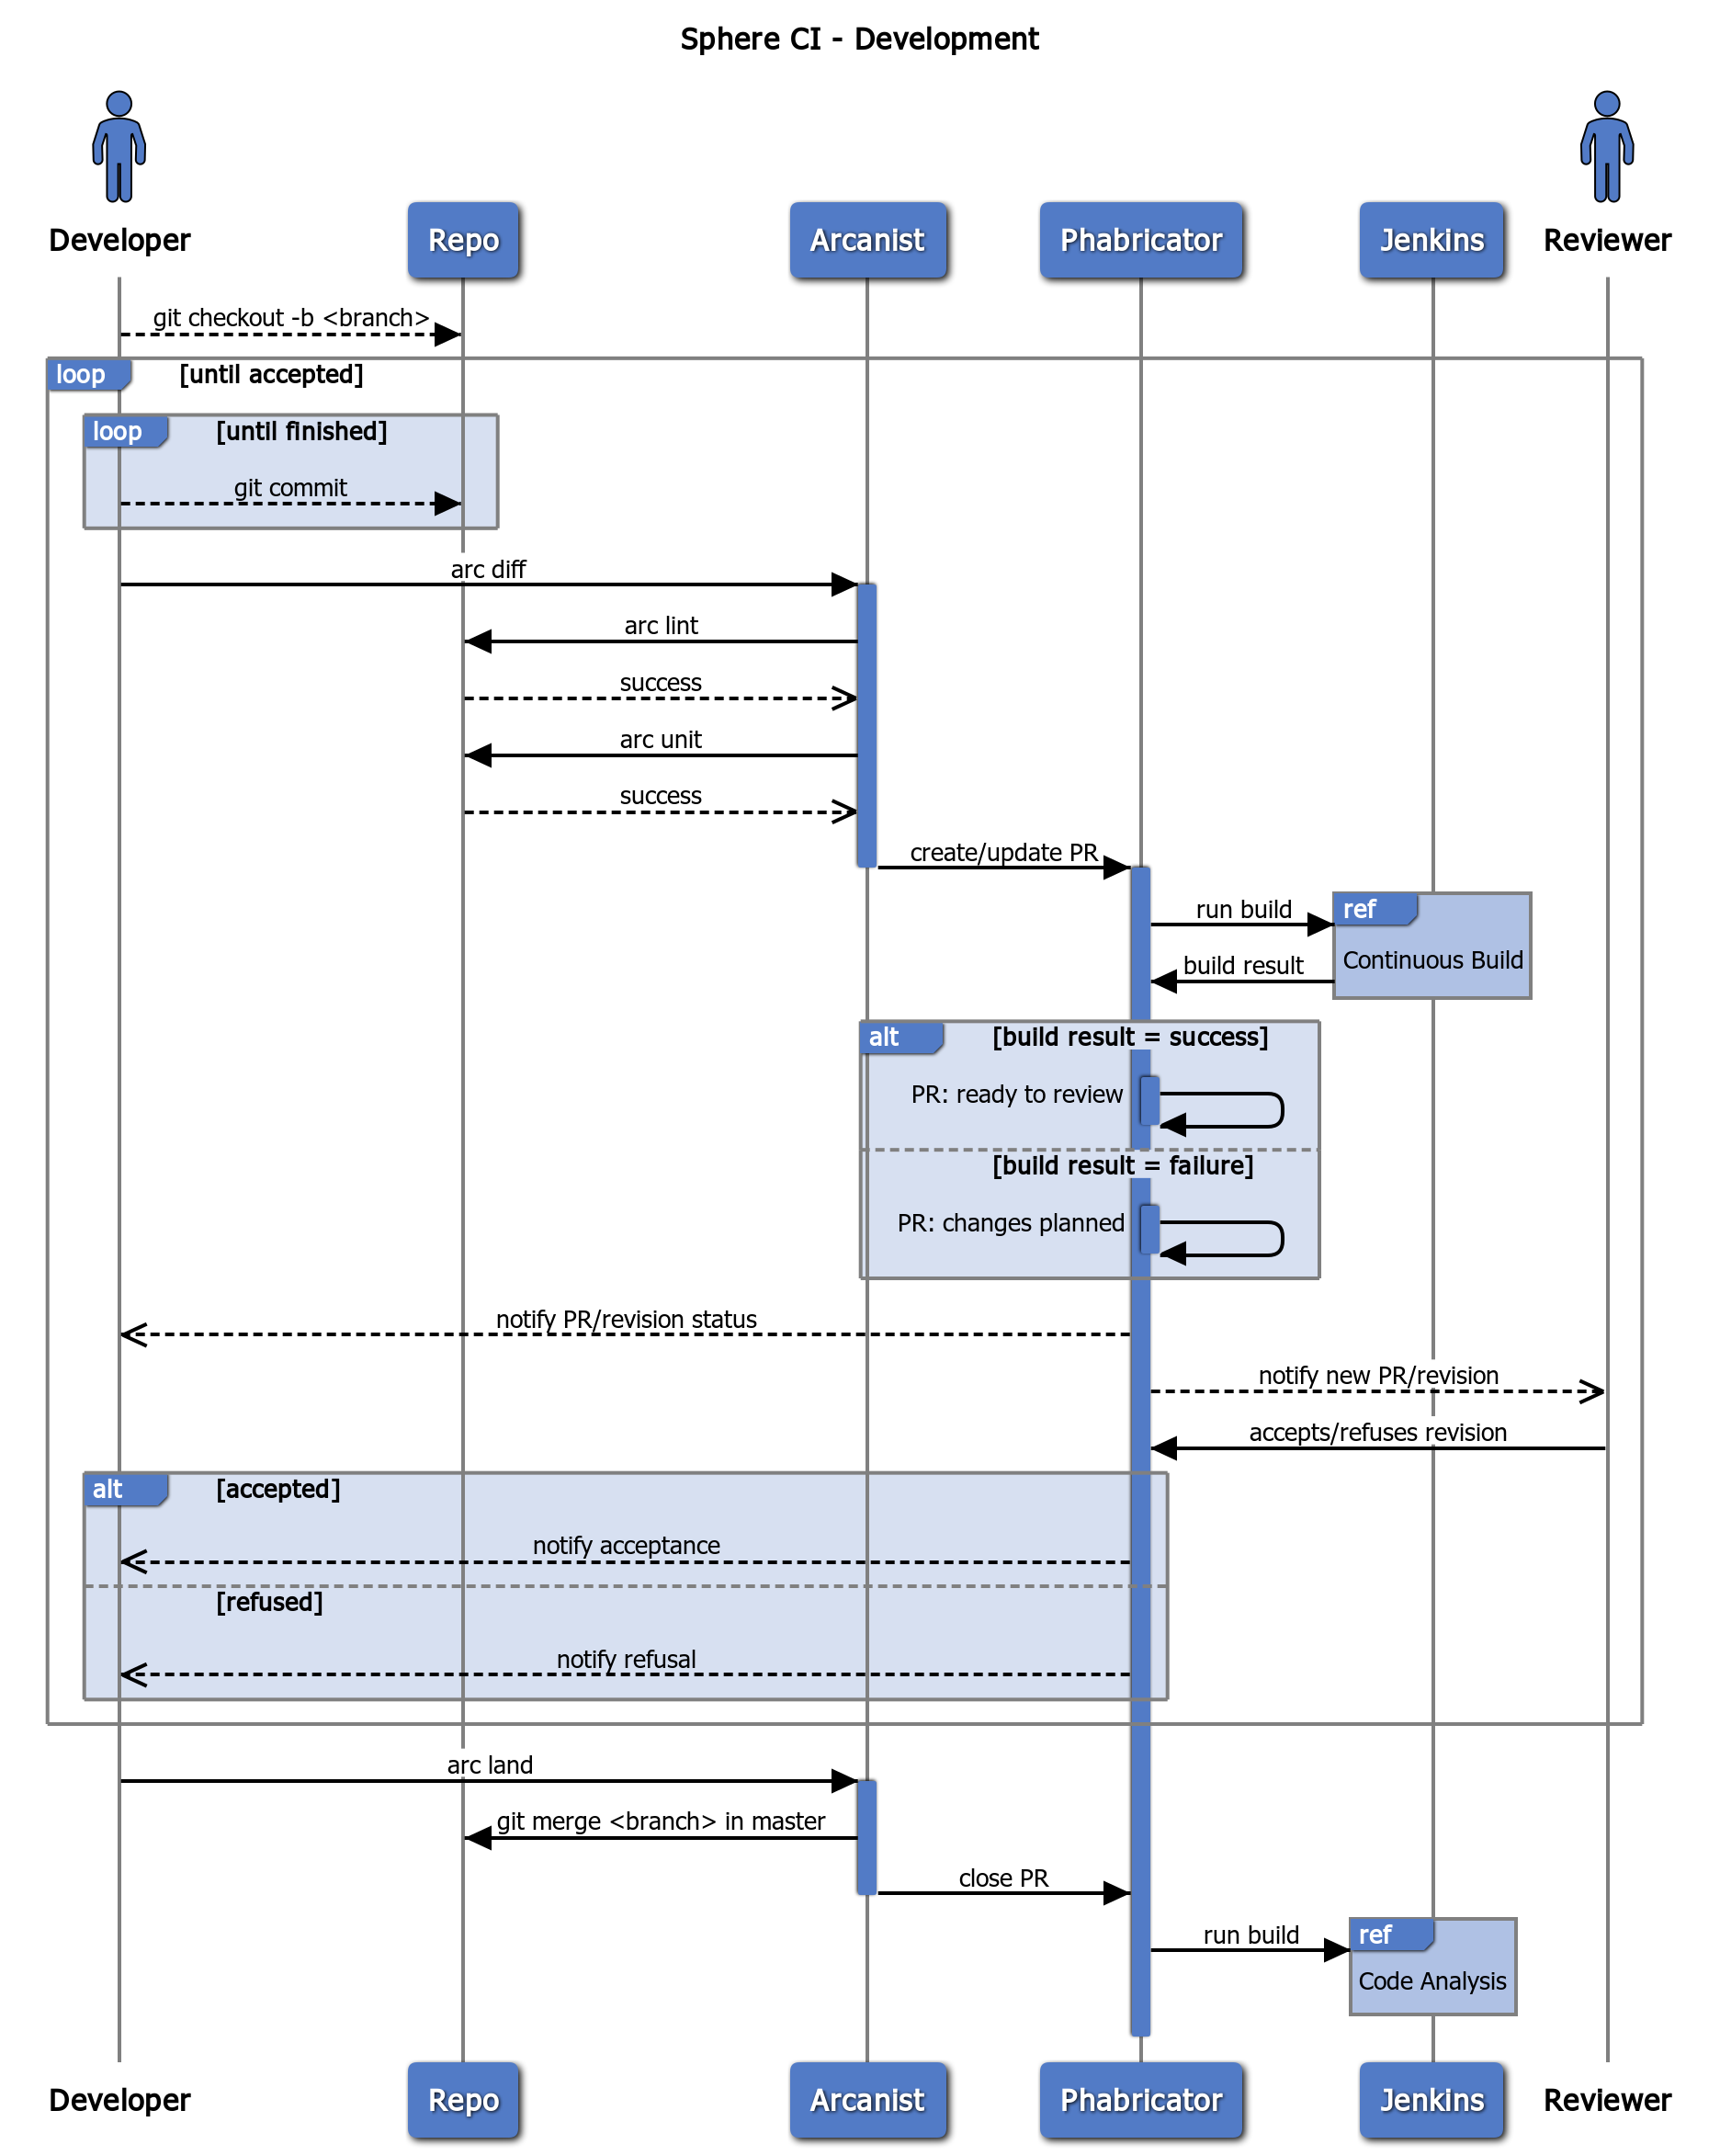
\includegraphics[width=\textwidth]{sphere_ci_dev}
        			\caption{Sphere CI - Development Flow}
        			\label{fig:sphere_ci_dev}
    	        \end{figure}
    	
    	    \subsection{\emph{Continuous Build}}
    	    
    	        \begin{figure}[H]
        			\centering
        			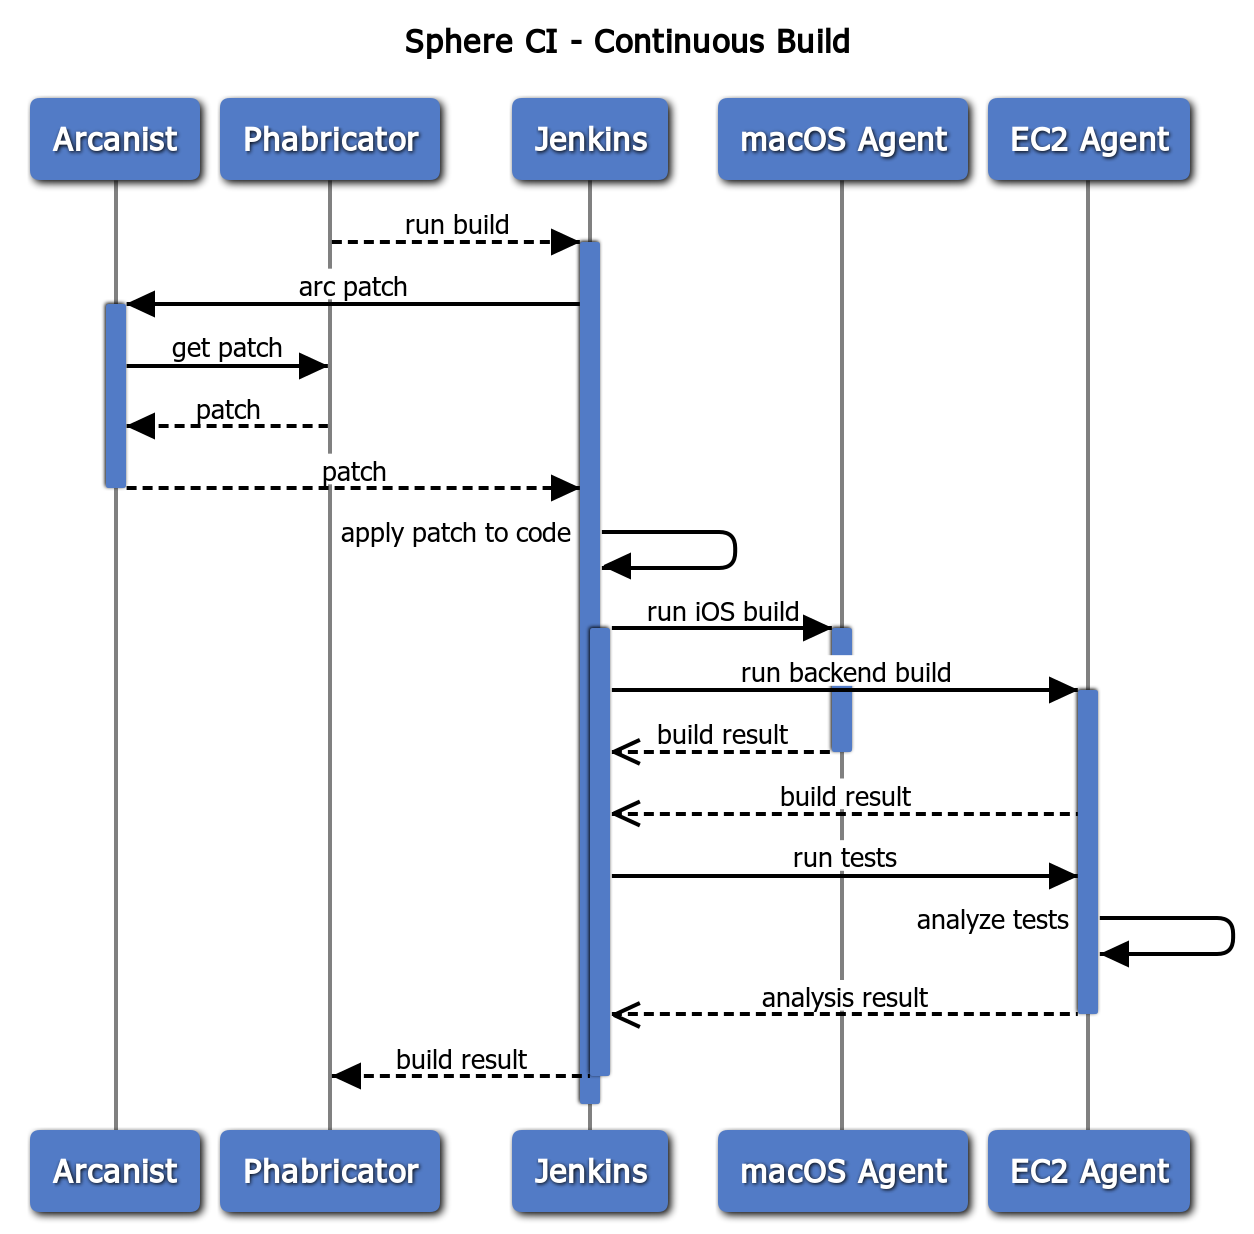
\includegraphics[width=\textwidth]{sphere_ci_build}
        			\caption{Sphere CI - Continuous Build}
        			\label{fig:sphere_ci_build}
    	        \end{figure}
    	        
    	    \subsection{Analisi del Codice}
    	    
    	        \begin{figure}[H]
        			\centering
        			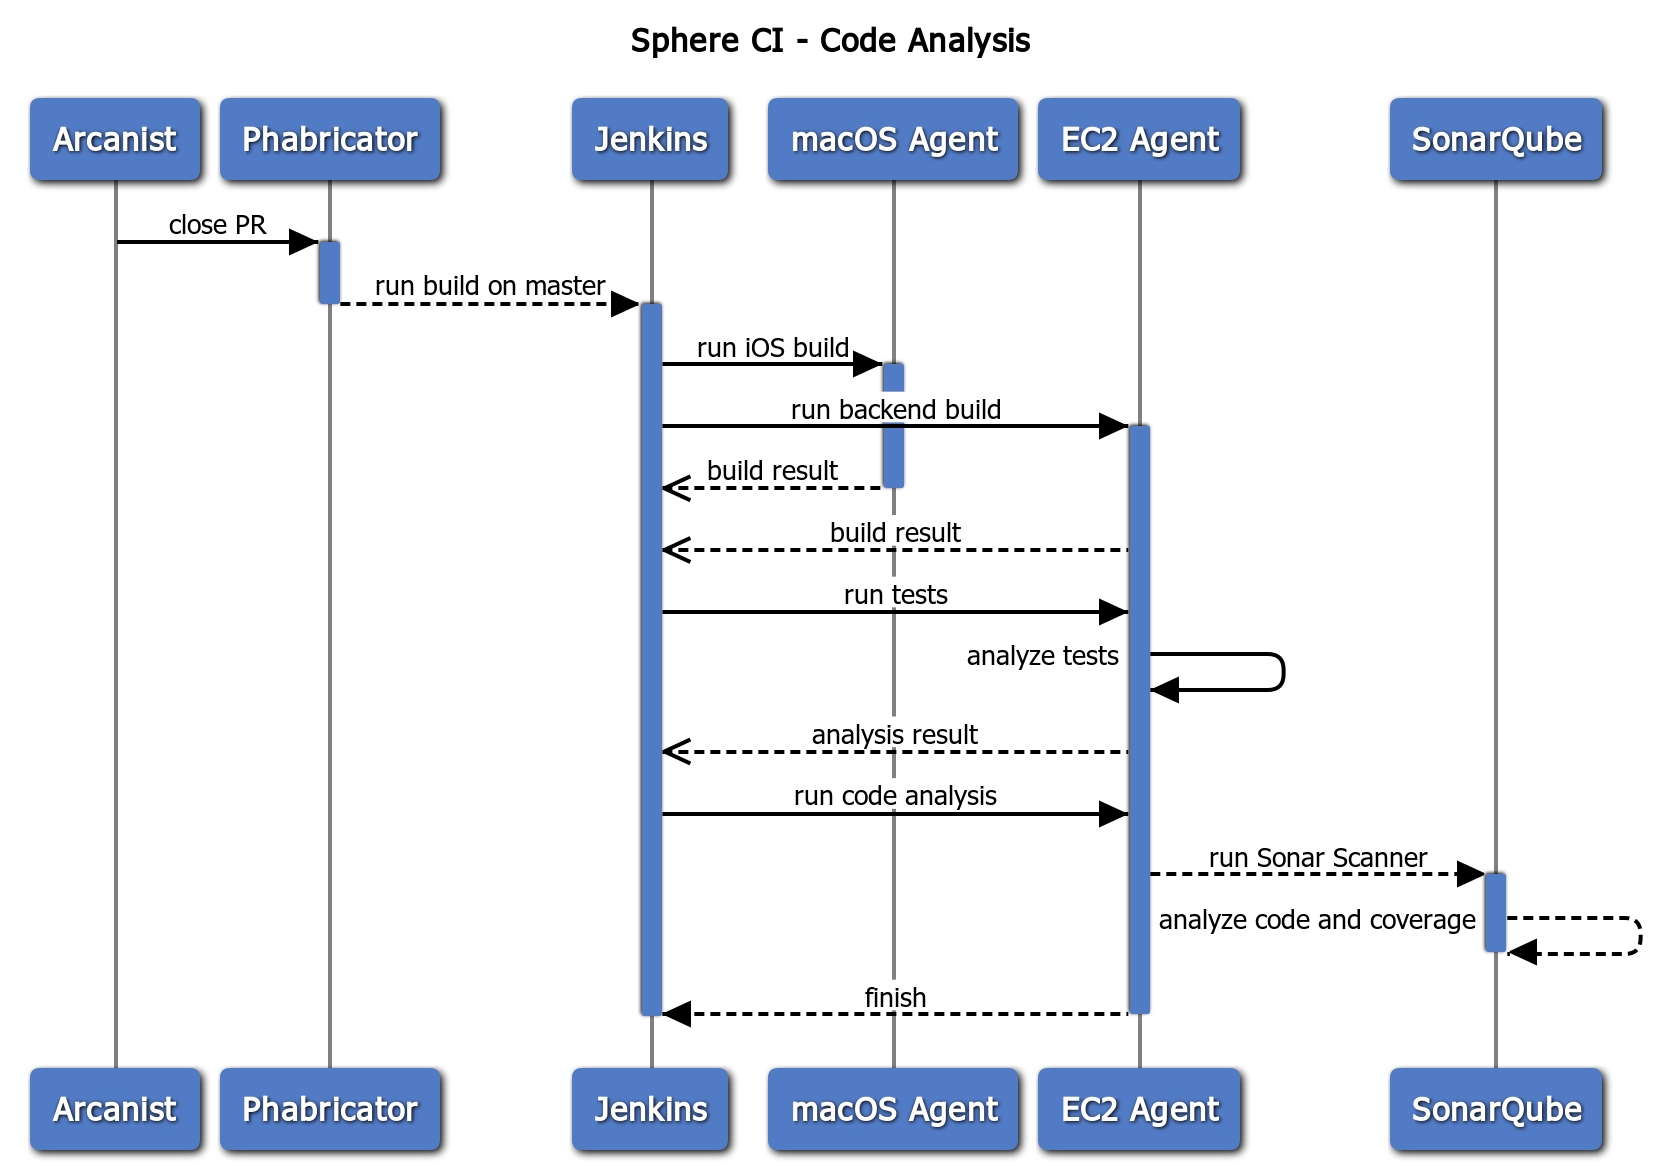
\includegraphics[width=\textwidth]{sphere_ci_code_analysis}
        			\caption{Sphere CI - Code Analysis}
        			\label{fig:sphere_ci_code_analysis}
    	        \end{figure}
    	
    	\section{Testing e Analisi del Codice}
    	
    	    \subsection{Unit e Integration Tests}
    	    
    	        L'esecuzione degli \emph{unit} ed \emph{integration tests} permette di rilevare problemi precocemente durante le prime fasi di revisione di una Pull Request. Tali tests vengono definiti in fase di sviluppo, integrati nel build system mediante definizione di regole relative a \emph{Bazel}, e poi eseguiti dal processo di \emph{Continuous Build} da Jenkins.\\*
    	        
    	        Il \textbf{Tests Analyzer Plugin}, illustrato in figura \ref{fig:jenkins_test_analyzer}, permette di aggregare, visualizzare ed analizzare l'andamento dei test in base alle build effettuate (le ultime 10 in questo caso), utilizzando una semplice interfaccia integrata nella schermata di pipeline su Jenkins. Per sfruttare questo plugin il formato di output dei test deve necessariamente essere \textbf{JUnit XML}, inoltre il plugin permette di visualizzare anche il \textbf{tempo di esecuzione} dei singoli test, individuando quelli che necessitano di ottimizzazione o \emph{refactoring} perchè troppo lunghi.
    	
    	        \begin{figure}[H]
        			\centering
        			\frame{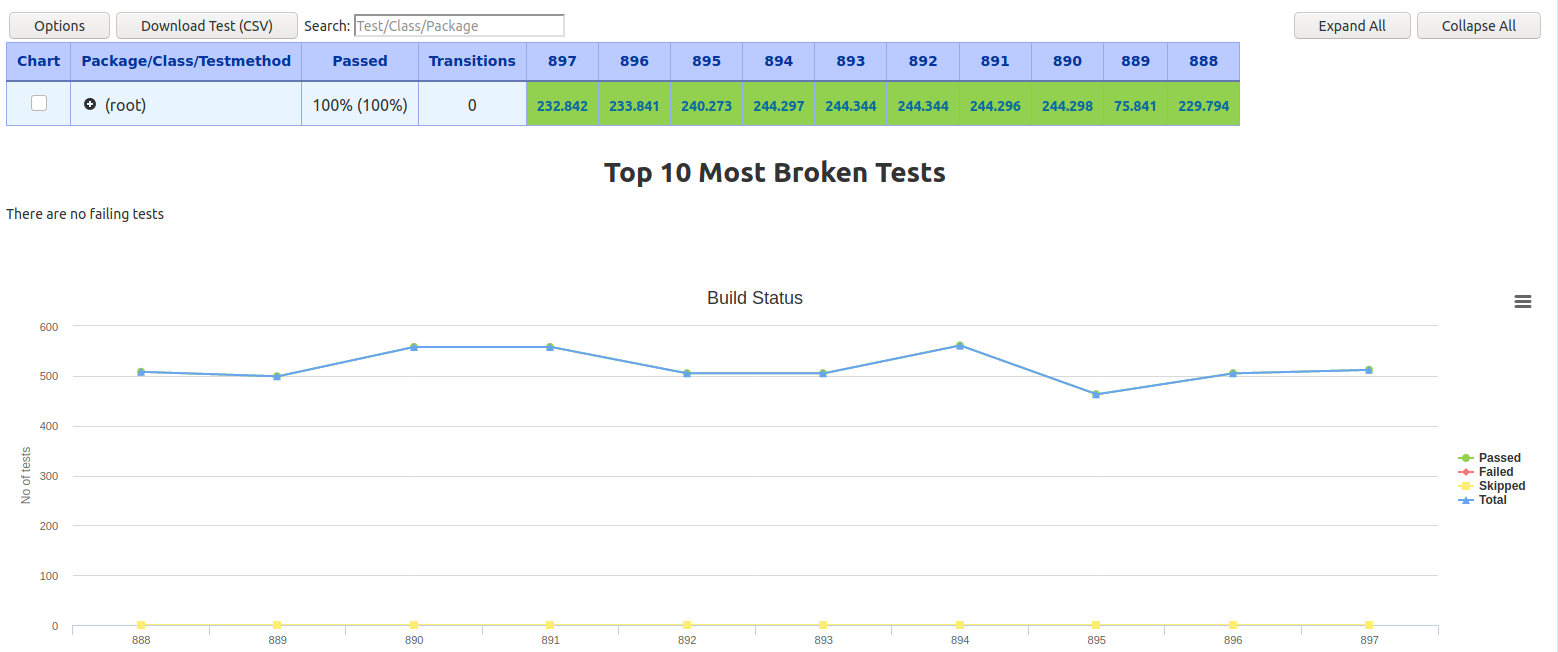
\includegraphics[width=\textwidth]{jenkins_test_analyzer}}
        			\caption{Jenkins - Tests Analyzer Plugin}
        			\label{fig:jenkins_test_analyzer}
    	        \end{figure}
    	
    	    \subsection{Code Coverage}
    	    
    	        Una analisi decisamente importante in fase di testing del codice è la \emph{Code Coverage}, ovvero quante righe di codice, \emph{branches} e rami sono stati coperti dai test definiti. Più è alta la coverage, più è possibile \textbf{scovare potenziali bug} avendo "scoperto" tutti i rami possibili del codice, ma \textbf{non indica la correttezza dei test} in se che potrebbero mancare di alcuni casi limite non gestiti neanche dal codice stesso.\\*
    	        
    	        Purtroppo, a causa di problemi durante l'implementazione della analisi di coverage sfruttando il build system scelto (Bazel) e a causa di bug e problemi interni allo stesso (file incompleti, necessità di dipendenze), \textbf{non} si è stati in grado di integrare con successo una analisi di \emph{Code Coverage} funzionante al momento della stesura di questo documento.
    	
        	\subsection{Quality Gates}
        	
        	    Per definire un livello di "qualità" del codice in SonarQube, vengono utilizzati i cosidetti \emph{Quality Gates}, ovvero soglie e definizioni create a priori che permettono poi a Sonar di definire se il progetto ha passato o meno quelle soglie, dando una idea generale della qualità del progetto stesso.\\*
        	    
        	    Prendendo come base il Quality Gate di default di SonarQube (chiamato \emph{Sonar way}), lo si è adattato semplicemente per integrare la mancanza di analisi della \emph{Code Coverage}, quindi eliminando la necessità che quel valore sia superiore all'80\%, come visibile in figura \ref{fig:sonar_quality_gate}. Il Quality Gate di default fornisce già da se una indicazione valida di qualità, dando come soglia minima un voto pari ad \textbf{A} per ogni parte della analisi di SonarQube, sotto il quale il controllo fallisce e bisogna reagire di conseguenza.
        	    
        	    \begin{figure}[H]
        			\centering
        			\frame{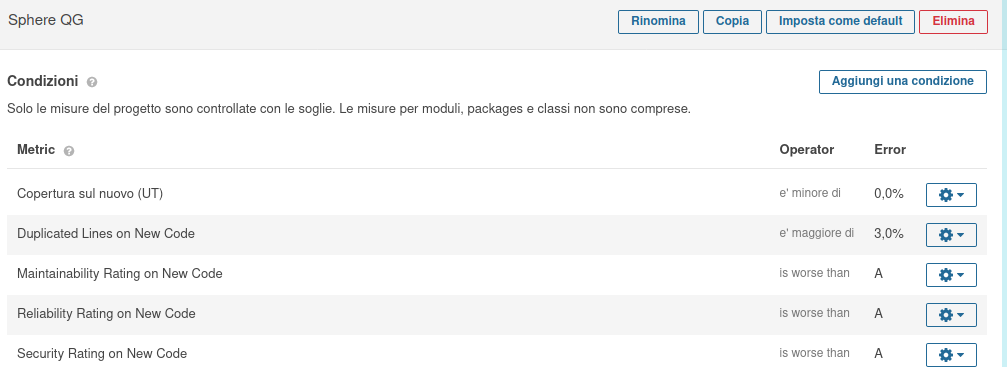
\includegraphics[width=\textwidth]{sonar_quality_gate}}
        			\caption{SonarQube - Quality Gate}
        			\label{fig:sonar_quality_gate}
    	        \end{figure}
        	
        	\subsection{Risposta a cambiamenti nella qualità}
        	
        	    A seguito di una analisi effettuata su SonarQube, il sistema potrebbe individuare potenziali bug, code smells, duplicazioni o indicazioni che potrebbero interessare o meno in base alla loro gravità.
        	    
        	    \begin{figure}[H]
        			\centering
        			\frame{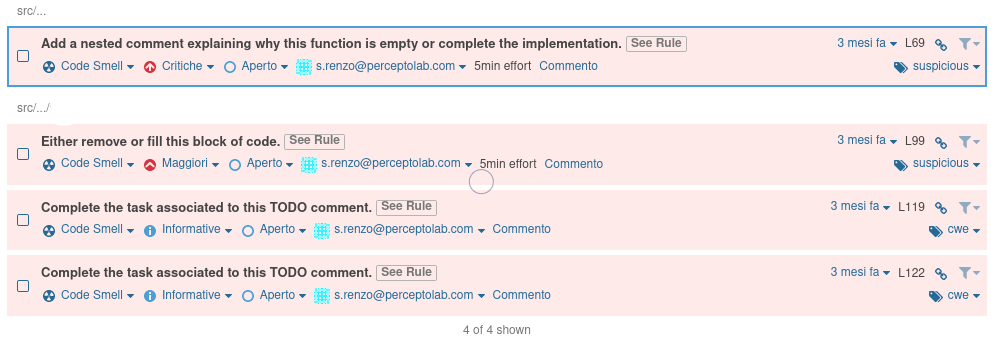
\includegraphics[width=\textwidth]{sonar_issues}}
        			\caption{SonarQube - Issues}
        			\label{fig:sonar_issues}
    	        \end{figure}
    	        
    	        Tali \textbf{issues} individuate da Sonar verranno \textbf{automaticamente assegnate} da risolvere \textbf{allo sviluppatore che le ha introdotte}, come definito dal sistema di versioning del codice (Git), mentre non verranno assegnate se l'analisi è stata effettuata per la prima volta e quindi non ha uno stato precedente con cui confrontare. Rimane compito dello sviluppatore controllare ad ogni \emph{merge} il risultato ottenuto dalla analisi di SonarQube, o in generale controllare le \emph{issues} a lui assegnate, da risolvere alla iterazione successiva o prima di sviluppi ulteriori che possano intaccare il codice analizzato. Un esempio di issues è visibile in figura \ref{fig:sonar_issues} dove sono presenti 4 issues pre-assegnate a chi le ha introdotte nel codice.
    	
    	\section{Risultati}
    	
    	    L'analisi dei test effettuati nel codice e l'analisi statica del codice ha permesso di ottenere una \textbf{migliore visibilità} di ciò che potrebbe impattare il progetto nel medio e lungo termine. Grazie alla integrazione di tutta la pipeline di \emph{CI} ora gli sviluppatori riescono a \textbf{risolvere preventivamente i problemi} che sorgono durante la compilazione, quando prima spesso si rischiava di unificare del codice che in realtà non funzionava, per poi accorgersene in fase troppo tardiva e risultava necessario agire per risolvere i problemi introdotti.\\*
    	    
    	    La facilità di utilizzo di tali analisi, mediante l'introduzione di uno strumento come Phabricator ed Arcanist, assieme ad uno strumento utilizzato in tutto il mondo come Jenkins, ha permesso quindi di \textbf{aumentare esponenzialmente la qualità del codice} prodotto, renderlo sempre più visibile a tutto il team che risulta così coinvolto attivamente nelle fasi di \emph{Code Review}, \emph{Continuous Build} e \emph{Code Analysis}.\\*
    	    
    	    Un guadagno importante è stato inoltre la \textbf{riduzione notevole nelle tempistiche di compilazione}, con guadagni nell'ordine del 300\% nei casi medi e fino al 500\% nei casi migliori, rispetto al processo legacy illustrato. Con il nuovo processo infatti non troviamo più colli di bottiglia dovuti alla compilazione dei servizi di backend, pur avendo più step e più operazioni nella pipeline, con lo step più lento (la build su macOS) che impiega circa 1.30 minuti nel caso migliore. L'unica casistica in cui si possono riscontrare rallentamenti è nella prima build della giornata, dovuti al \emph{cold start} delle istanze \emph{agent} create da Jenkins.\\*
    	    
    	    Riprendendo infine gli obiettivi iniziali prefissi, ed applicandoli al processo di \emph{Continuous Integration}, possiamo stilare una tabella di conseguimento che denota il loro raggiungimento completo (con tutte le variabili del caso):
    	    \begin{table}[h]
    	        \centering
    	        \begin{tabular}{ |p{9cm}||p{3.5cm}|  }
                    \hline
                    \textbf{Obiettivo} & \textbf{Raggiungimento} \\
                    \hline
                    Analisi dei Requisiti per i processi CI & \cmark \\
                    Pipeline di CI per i servizi di Backend e Mobile & \cmark \\
                    QA basato sulla analisi dei test e del codice & \cmark \\
                    Infrastruttura basata su AWS per gestire il processo & \cmark \\
                    \hline
                \end{tabular}
    	        \caption{Sphere - Raggiungimento Obiettivi CI}
    	        \label{tab:sphere_obj_ci}
	        \end{table}

        \section{Esperienza Applicativa}

            Durante il corso del design ed implementazione della pipeline di \emph{Continuous Integration} vi sono state diverse modifiche nell'approccio ad uno dei problemi fondamentali, ovvero i tempi di compilazione.\\*
            
            Partendo come spunto dal processo legacy precedente, si era provato inizialmente a \textbf{riutilizzare} il servizio di \textbf{AWS CodeBuild} con poco successo, anche sfruttando i sistemi di caching remoto o tramite file system, a causa della astrazione che fa il sistema non si poteva garantire l'utilizzo della stessa macchina e quindi dello stesso ambiente. Questo fatto causava problemi a Bazel che spesso e volentieri ricompilava intere dipendenze per un cambio solo dell'ambiente di build, allungando le tempistiche al pari del processo precedente.\\*
            
            Un altro problema sorto durante lo sviluppo è stata la \textbf{connessione VPN} utilizzata sull'\textbf{Apple Mac Mini}, inizialmente gestita a livello di client nel sistema operativo, che frequentemente si disconnetteva e faceva fallire delle build avviate da Jenkins specialmente nelle fasi iniziali (ma dopo lunghi timeout). A seguito di un ammodernamento dell'infrastruttura di rete \emph{on premise}, si è poi spostata la connessione VPN a livello di router, eliminando così questa variabile e risolvendo definitivamente il problema.\\*
            
            Il resto del processo è stato visto essere molto solido e ben riutilizzabile indipendentemente dal progetto, o con minimi cambiamenti dovuti più all'ambiente di compilazione che al processo in se. Punto interessante è di sicuro l'\textbf{integrazione locale con Arcanist}, l'unico vero punto dipendente dal progetto poiché \textbf{sfrutta Bazel} per effettuare le sue analisi, rendendo più difficoltosa l'integrazione con altri progetti (ma già effettuata con build system differenti con successo e poco effort).

\end{document}